%==================================%
\section{クボタアツム、大魔神説浮上}
%==================================%
それは、2015年某日の事、全てはATMのカスから生まれた。\par
研究室を出てすぐの広間で昼飯を食べていたオガワマンと(ポ)の前を、偶然ATMが通りかかった。オガワマンがATMに「おすすめのアーティスト教えてください」と問いかけた、ATMはこう答えた。
 \begin{center}
   「藤岡ヒロシ、」
 \end{center}
名前は聞いたことがあった我々だが、実際に曲を聞いたことがなかったので一応聴いてみることにした(図\ref{hirosi})。
ここで注目すべきはその曲名である。一般的な人間は簡略化して『娼本(ヨネポン)』と呼んでいるが、正式には \\

\fbox{
  \begin{tabular}{c}
    「ヨネモンGetだぜ!いけ!フシギダネ!」\\
    「曲名とは?」\\
    「それはッシャァァ〜!」\\
    「ダネフッシャ〜!」\\
    「上記で曲名は終わりでよろしい?」\\
    「いや、まだだ。」\\
    「なぜ終わりだと思ったのか?」\\
    「そうだそうだ、終わりだと思った理由を述べよ」\\
    「曲名がワンフレーズで終わるという時代はとうに過ぎた!」\\
    「世は大航海時代!探せぇ」\\
    「次回!アバポンヌ船長、宝を見つける!」\\
    「最終回!アバポンヌ船長、宝を見つけたとの虚偽の申告により逮捕、起訴、釈放」
  \end{tabular}
}\\

である。曲名からも伝わる、まさに名曲である。\par

\begin{figure}[H]
\centering
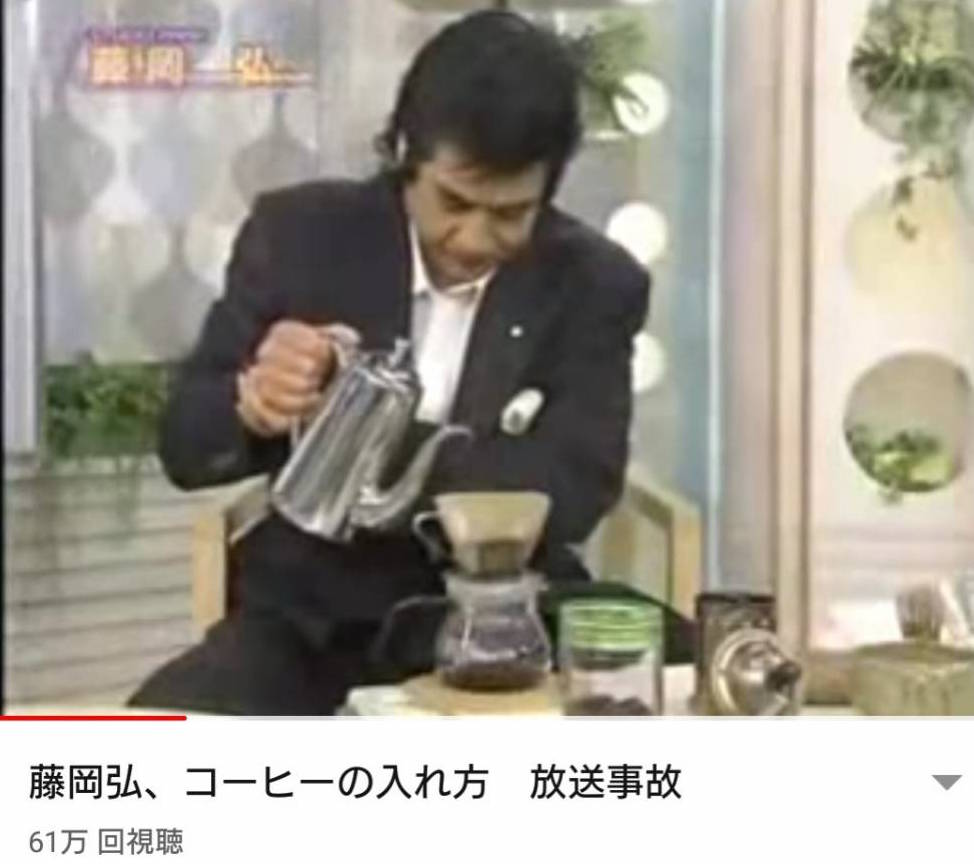
\includegraphics[clip,scale=0.2]{hirosi.jpg}
\caption{後の伝説となった藤岡ヒロシ、の名曲。オリコンチャート百億万年連続位の大ヒットとなる予定とのこと。}
\label{hirosi}
\end{figure}

この名曲の映像を見ていた時、事件が起こったのである。ATMが推してきた楽曲のMV(図\ref{hirosi})を見ていた時、オガワマンはあることに気づき、放った一言が事態を急変させる。
 \begin{center}
   「あれ、今のやつ中学校の同級生の大魔神に似てね?」
 \end{center}
この瞬間、即座にタケダ警察24時が設立され、世紀の大戦犯を逮捕すべく、世界規模の大捜索が始まった\footnote[1]{余談だが、オガワマン大魔神宣言の直後にATMが「確かにクボタアツムは京都出身のCカップやなあ」と証言していたのはまた別のお話。しかもこれでいて推しメンはまた別というキモさ。}。\\
 それからというものの、どう考えても明らかにおもしろすぎる事案であるが、オガワマンの中学でのカスかな記憶では「大魔神はこんな藤岡ヒロシ、になるようなキャラじゃなかった」という固定概念があり、創作の邪魔をすべくアリバイ工作に奔走していくのである。
\par

しかし、その努力も虚しく、徐々にその証拠は集められていく。基本的に、その時々の捜査段階で、オガワマンは今回のクボタアツムと大魔神の一致精度を標準偏差$\sigma$で評価している。この大捜索が開始された段階では1$\sigma$であった。当たり前である。これに対し、完全一致を確信しているタケダ警察は約2年に及ぶ大捜索の末、少しばかりの証拠が得られた。ここでそのほんの少しの証拠達を以下に示す。
\begin{itemize}
\item まず顔が似てる
\item 声も似てる(調査開始後1秒時点)
\item 出身地が同じ都道府県(調査開始後数秒後時点)
\item 誕生日は誤差1日以内(調査開始後数日時点)
\item 中学の頃の部活が吹奏楽で一致(調査開始後数ヶ月時点)
\item 中学の頃の部活の担当楽器が一致
\item 部活で脚の怪我をしたこととオガワマンの記憶が一致
\item 部活で脚の怪我をした箇所と、オガワマンが所持する卒アルに載ってる写真で、怪我と同時期に撮影された写真に写る怪我している場所が一致
\item オガワマンが成人の日の同窓会で会った時の髪型と、YouTubeにuploadされたOfficial動画にて「成人式に来ました」と言ってる時の髪型が一致
\end{itemize}

まあ、$3\sigma$と言ったところである。$\sf{ (´\_ゝ`)}$笑\par
まあ、捜査の努力に免じて$4\sigma$でもいいけどな$\sf{ (´\_ゝ`)}$笑\par
頑なに$5\sigma$まで認めないオガワマンであったが、それと同様に、当初から常々「本人に確認しない限り$5\sigma$は認めない」と言っていた。
そして、世紀の大捜索から早2年、後の伝説となる「直接対決」が実現することとなる。
\par
果たして、$5\sigma$に到達することができるのか、乞うご期待っっっっっっっ
